\documentclass[12pt]{article}
\usepackage[a4 paper, portrait, margin=0.75in]{geometry}
\title{EGYPT\\Farmers to Pharoahs}
\author{Derrick Diana\\Harry Heathcock\\Kaedon Jon Williams}
\date{\today}
\usepackage{multicol}
\usepackage{graphicx}
\usepackage{indentfirst}
\graphicspath{ {Figures/} }

\begin{document}
	\maketitle
	\begin{abstract}
			
	\end{abstract}
	
	\section{Introduction}
		\subsection{Changes}
			A number of changes in the implementation were made, some due to what seemed to be implementation errors in the original code and others due to functionality not making sense with what was trying to be achieved. Those which affect functionality have been implemented as explained, however when the Legacy Mode setting is enabled, these changes are reverted back to how they were in the original implementation.
			\subsubsection{Death Due to Lack of Grain}
				In the original NetLogo code, if a household did not have enough grain to survive a year then a single person would die and the grain would be set to zero. In reality this doesn't make sense, as if a household has no food, then no one would survive. The reimplementation changed this so that only the family members who can be fed will survive.\\
			\subsubsection{Population Increases}
				In the original code, if the total current population is less than or equal to the historical projected population then the population can increase. At first glance this seems to be correct, however this allows the population to always grow slightly faster than the projected historical value, and thus in the reimplementation this is changed so that the population will only increase if it is less than the historical projected population.\\
			\subsubsection{Generational Changes in Ambition and Competency}
				In the original code, if the ambition or competency for a household moved out of the bounds set (minimum, up to 1) then a new value would be generated until it fell within the bounds. This means that the computational time for the ambition and competency changes are unbounded. In the reimplementation, a value within the possible range is generated.\\
			\subsubsection{Order of Field Claimants}
				In the original code, households claimed fields in ascending order of how much grain they currently have. This seemed inconsistent with every other operation being independant of grain or ordering, in the reimplementation, this ordering is randomised each year.
	\section{Screenshots}
		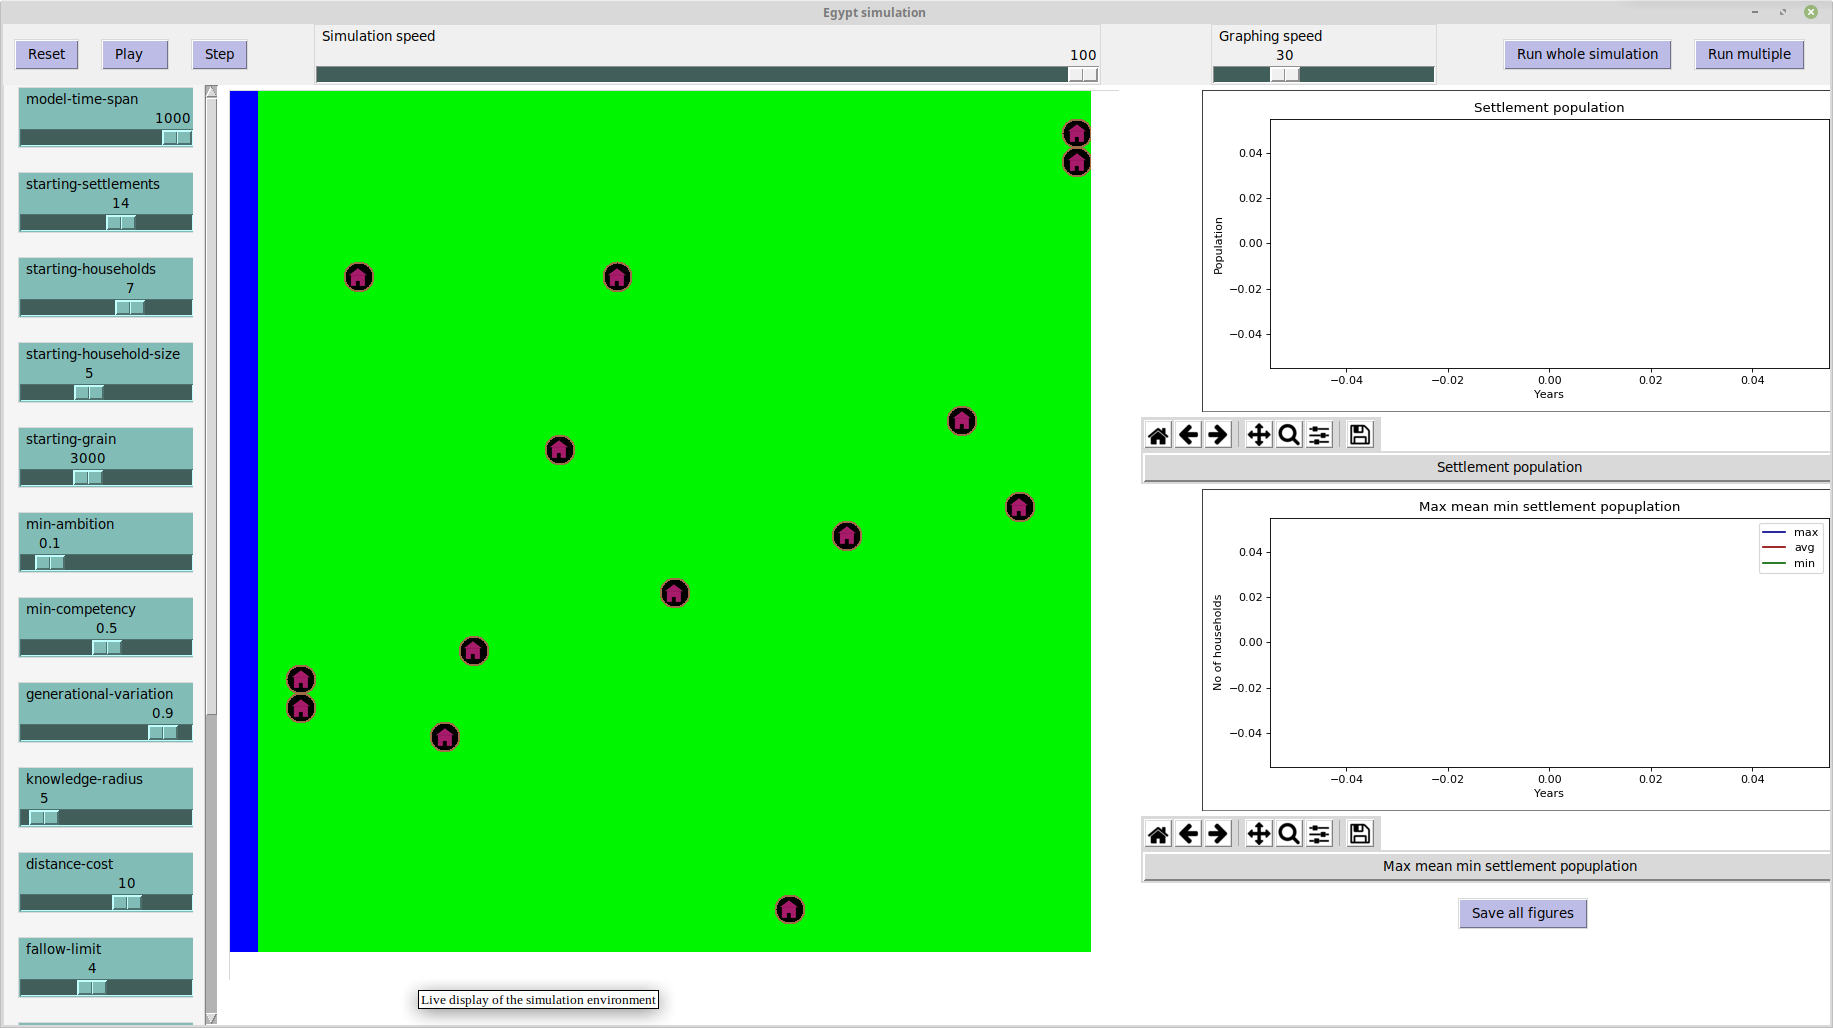
\includegraphics[width=\linewidth]{OnOpen}
		
		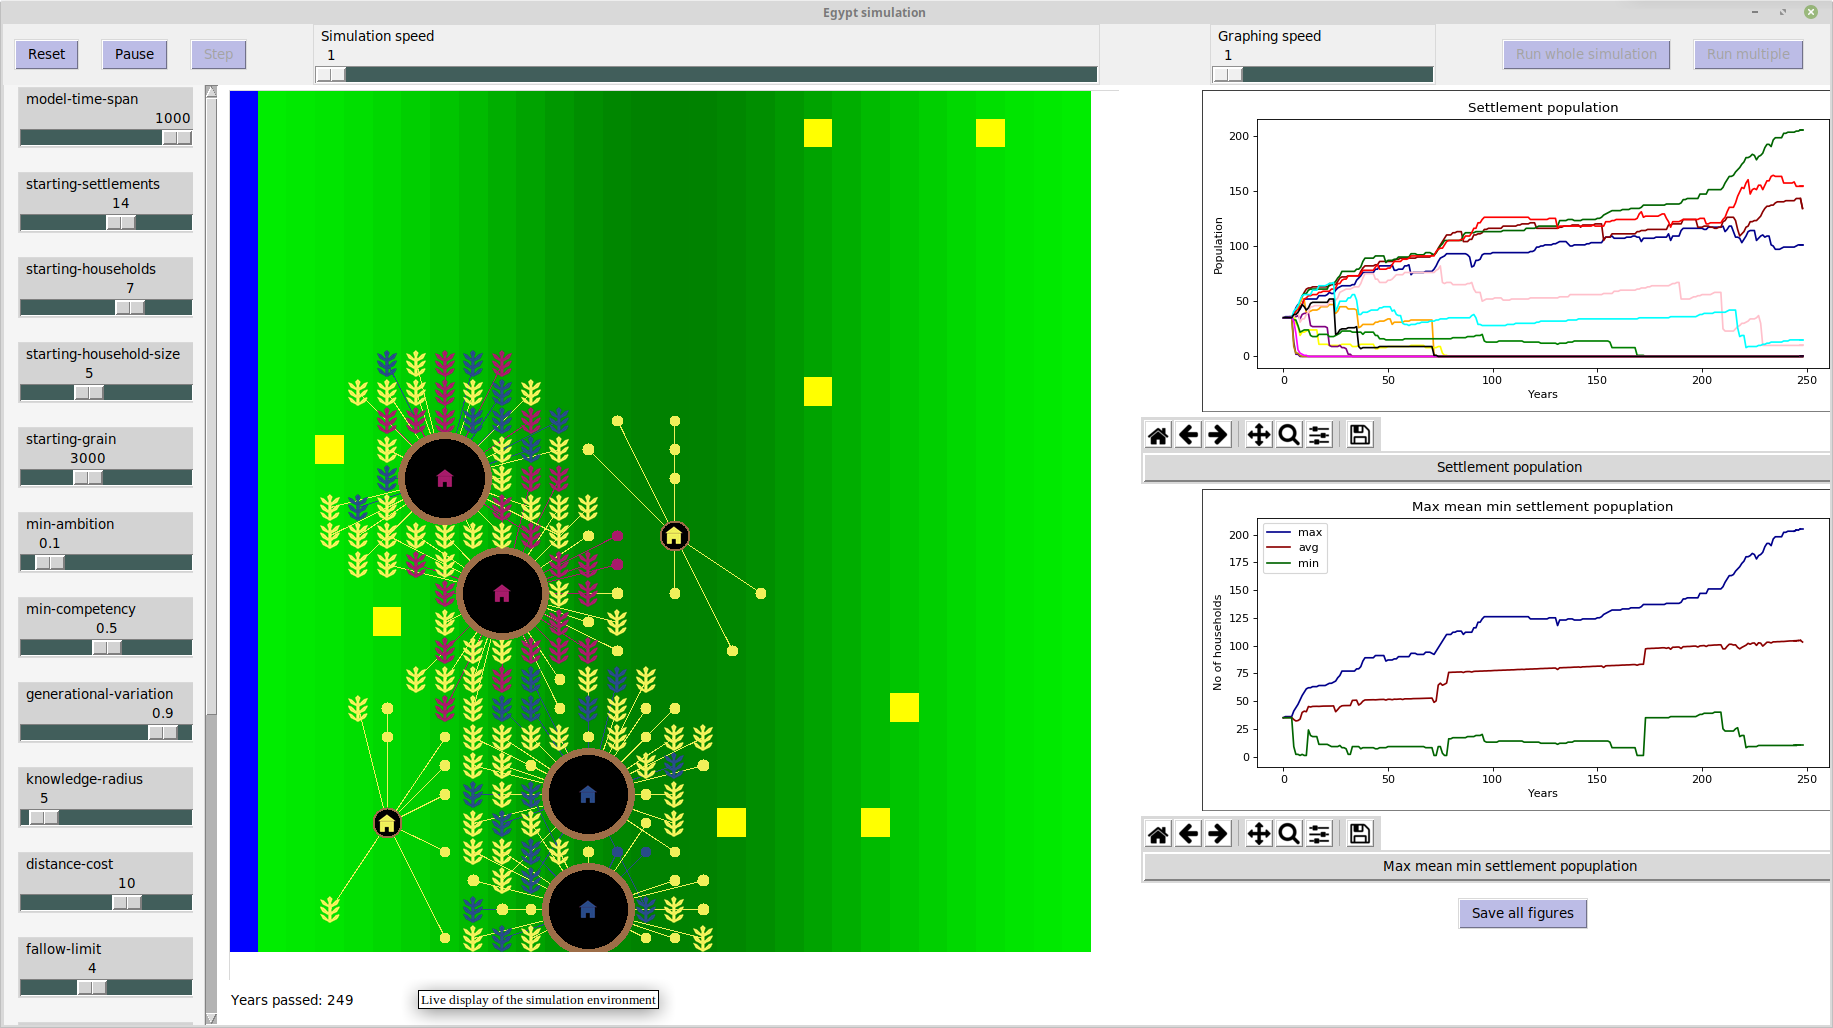
\includegraphics[width=\linewidth]{WhileRunning}
		
		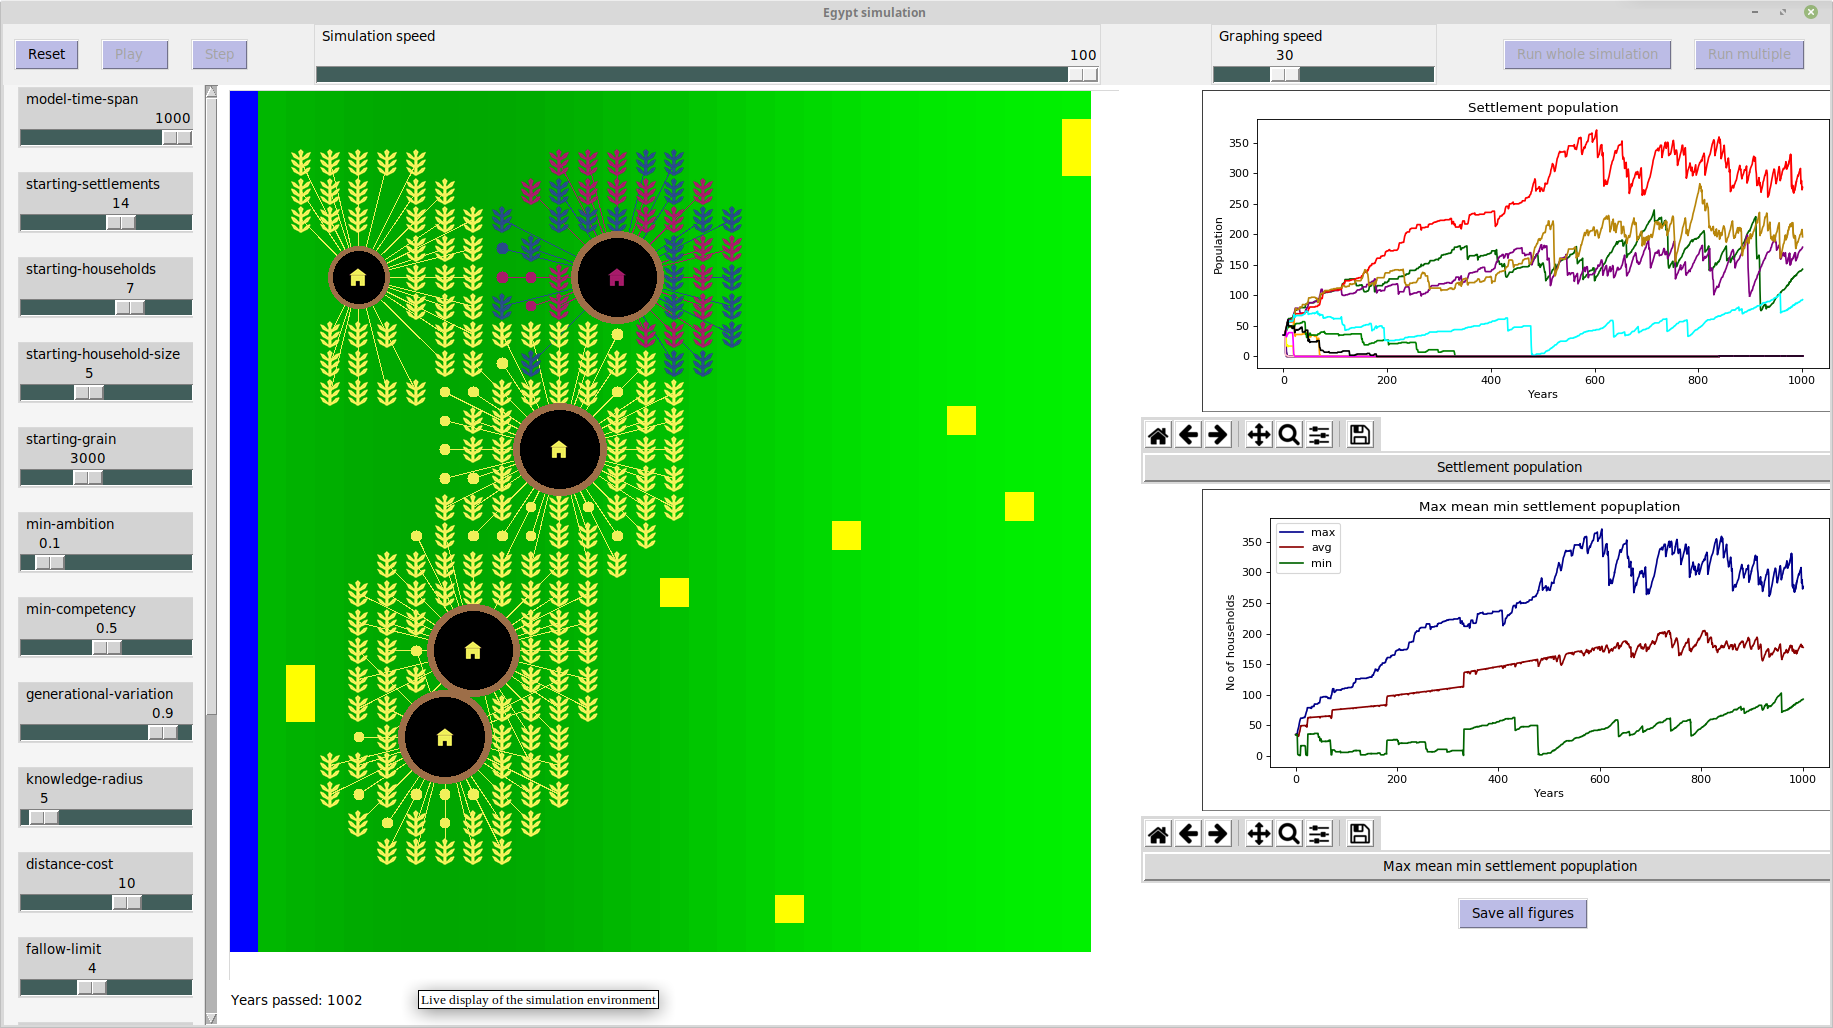
\includegraphics[width=\linewidth]{FinishedRunning}
		
		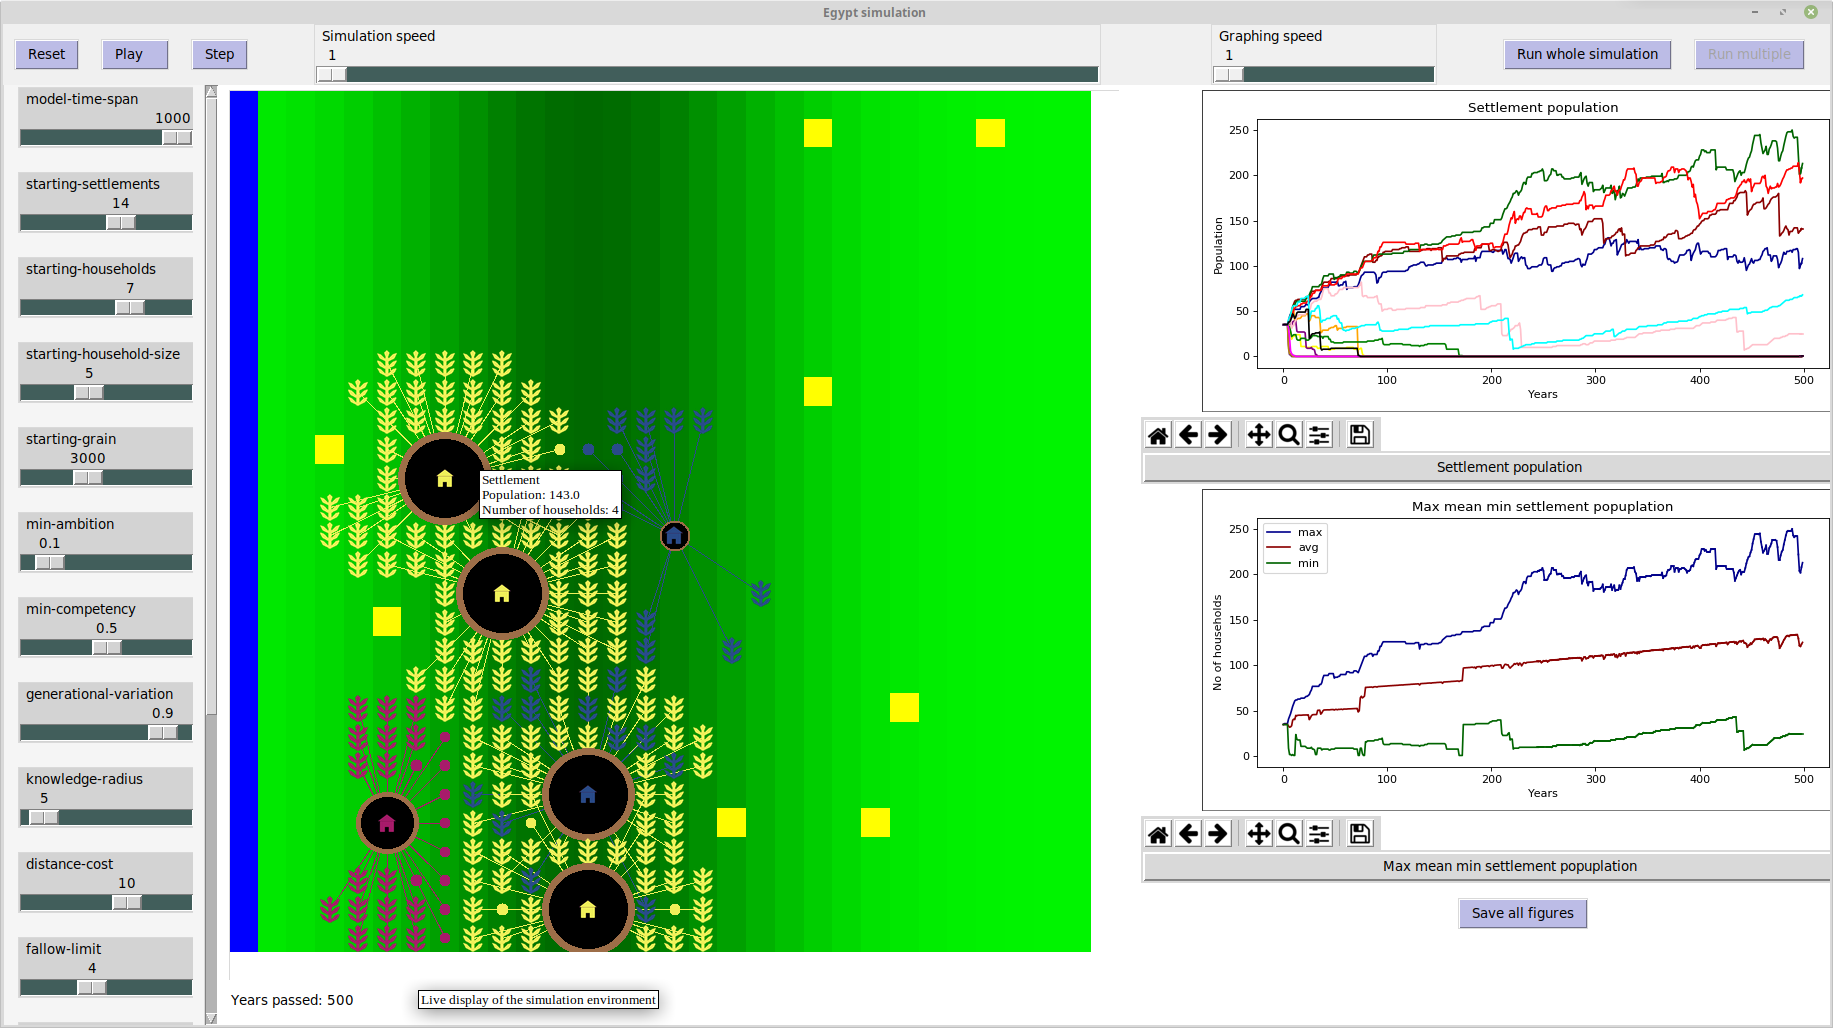
\includegraphics[width=\linewidth]{RightClickOnSettlement}
		
		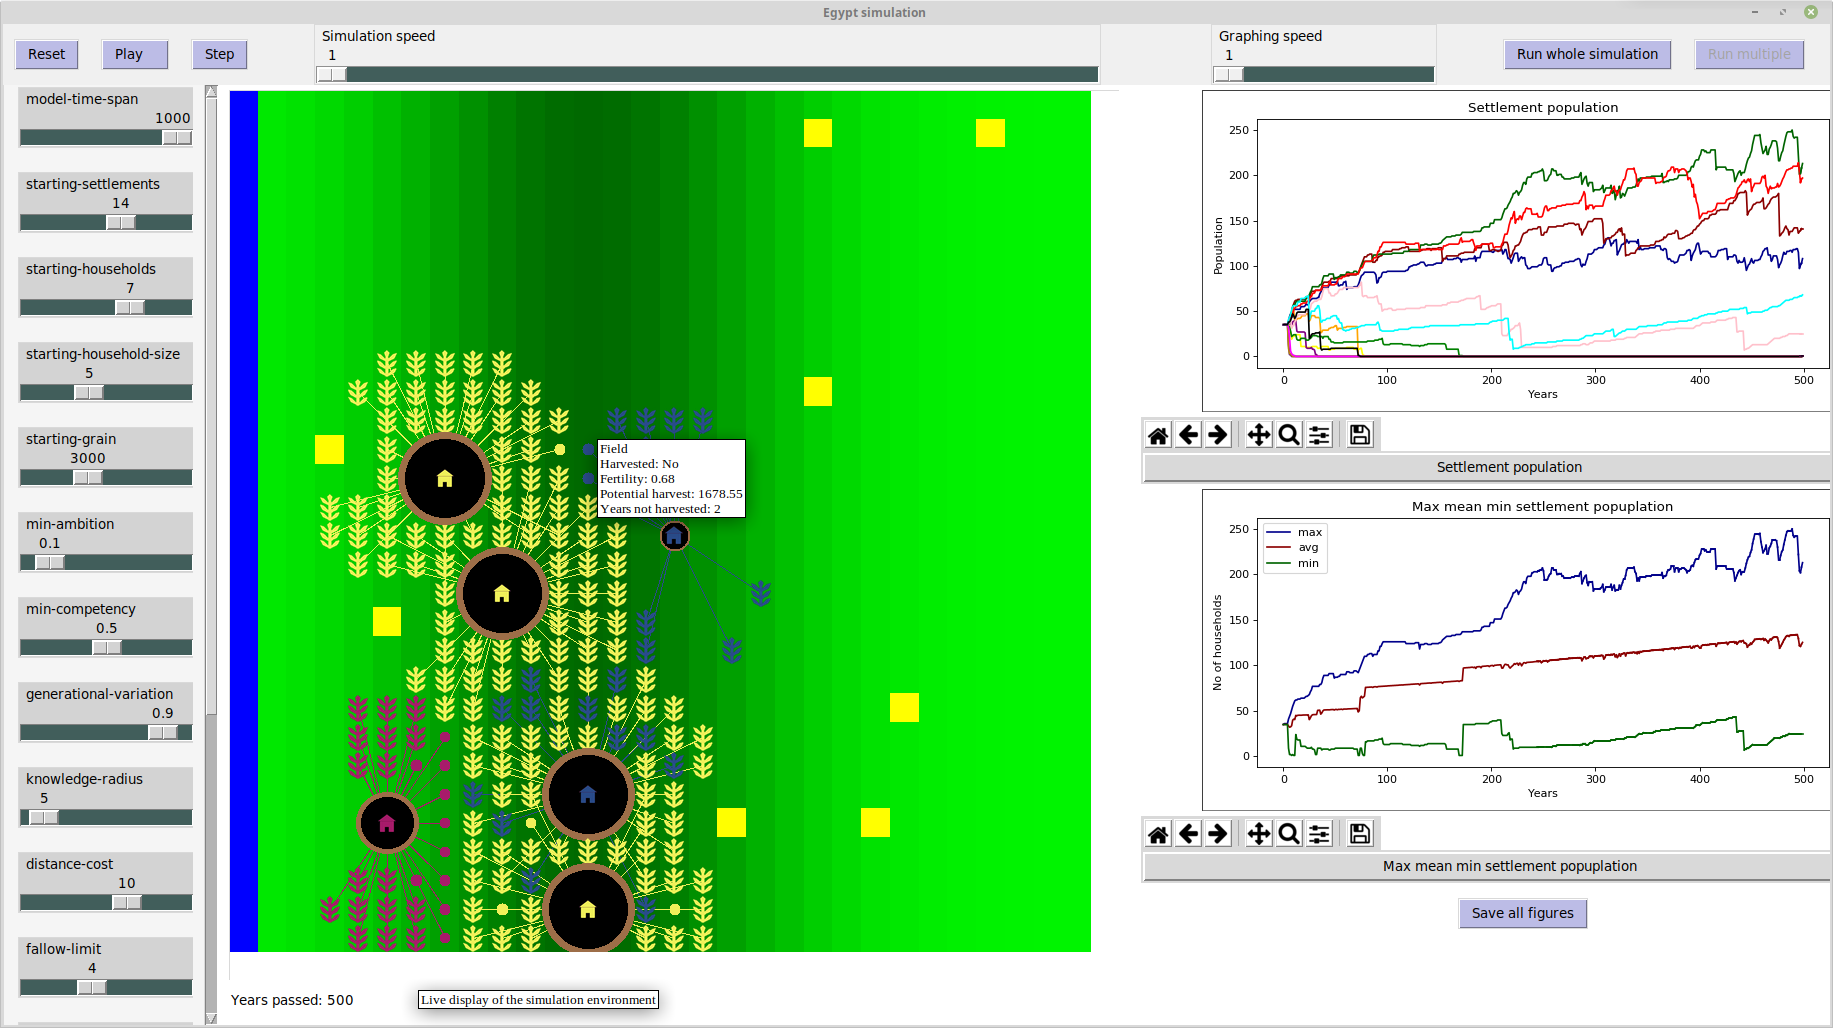
\includegraphics[width=\linewidth]{RightClickOnNotHarvestedField}
		
		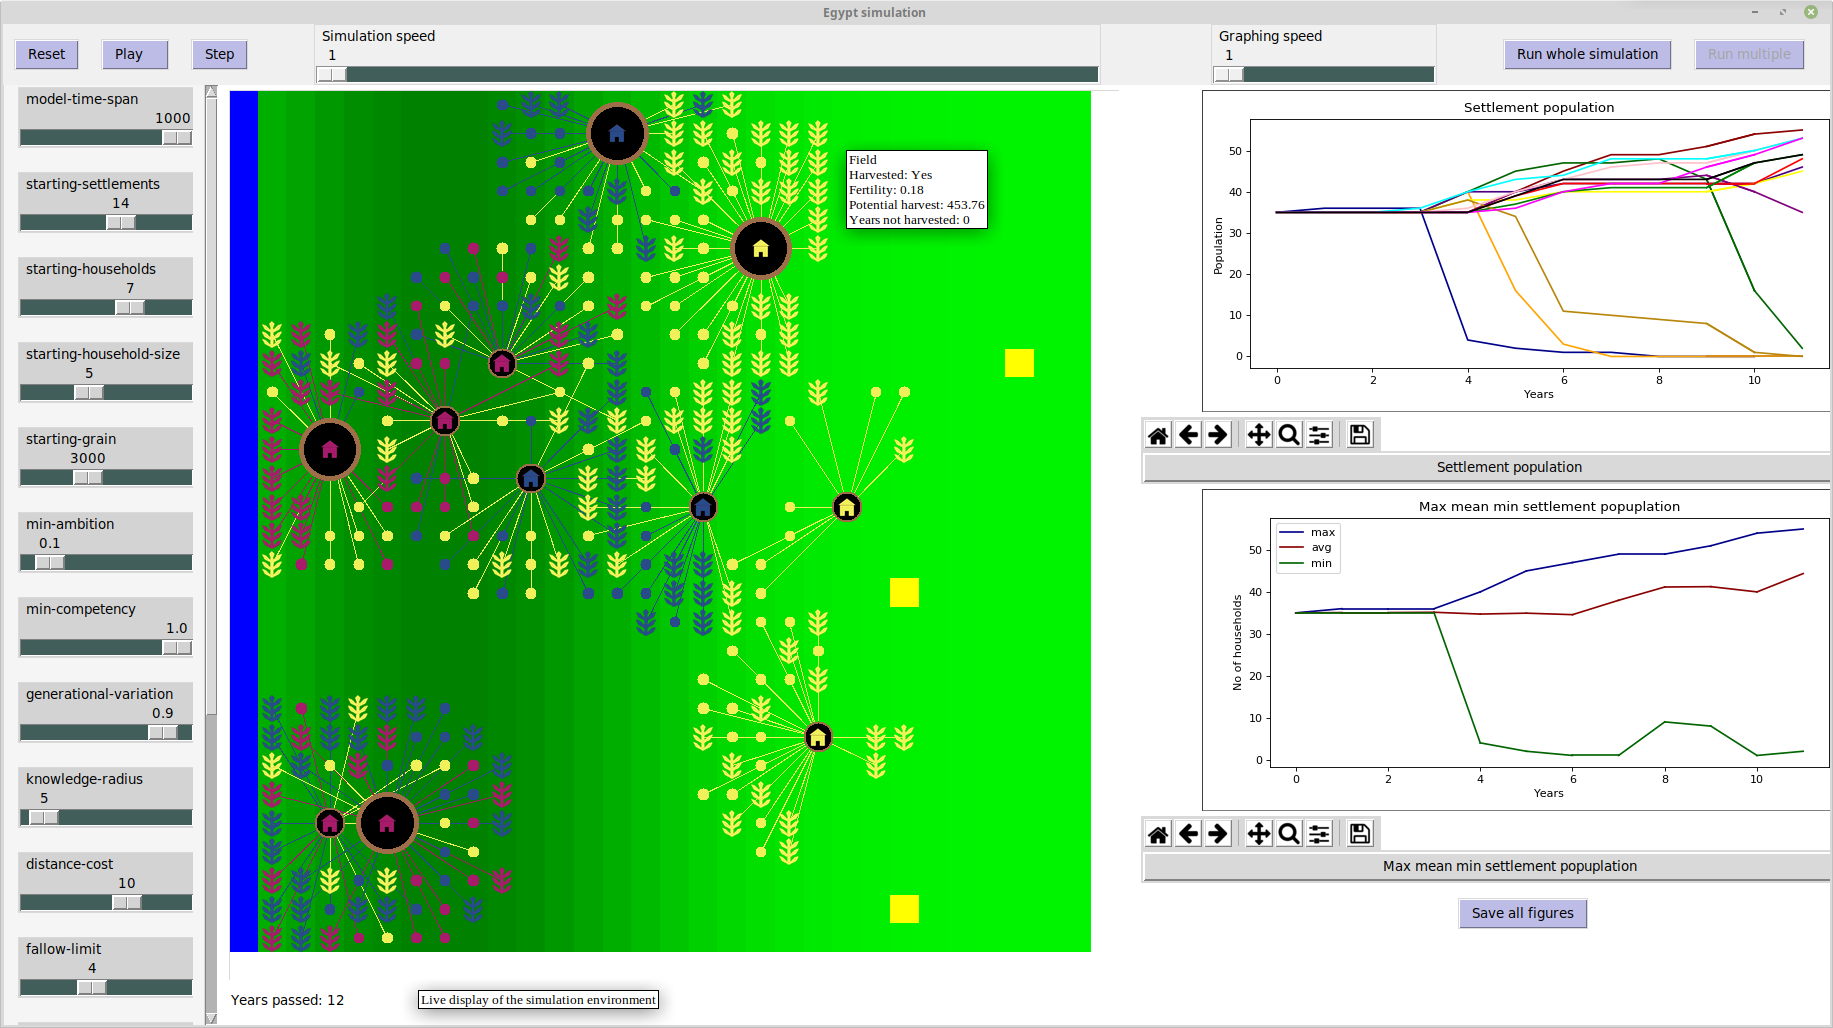
\includegraphics[width=\linewidth]{RightClickOnHarvestedField}
		
		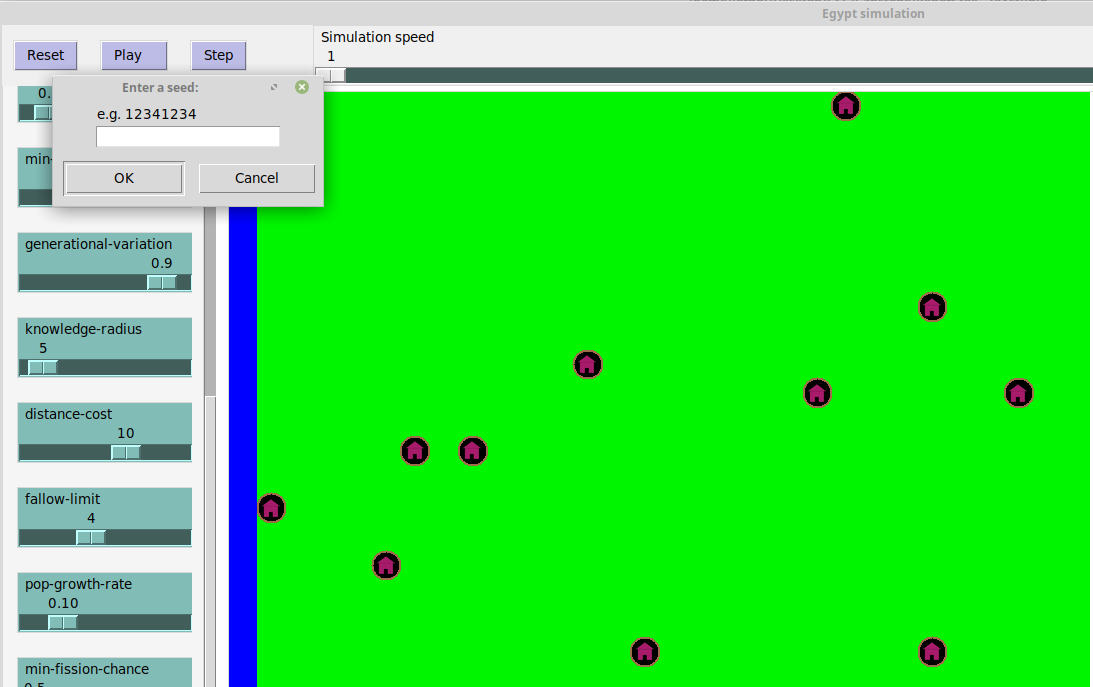
\includegraphics[width=\linewidth]{SeedEntry}
		
		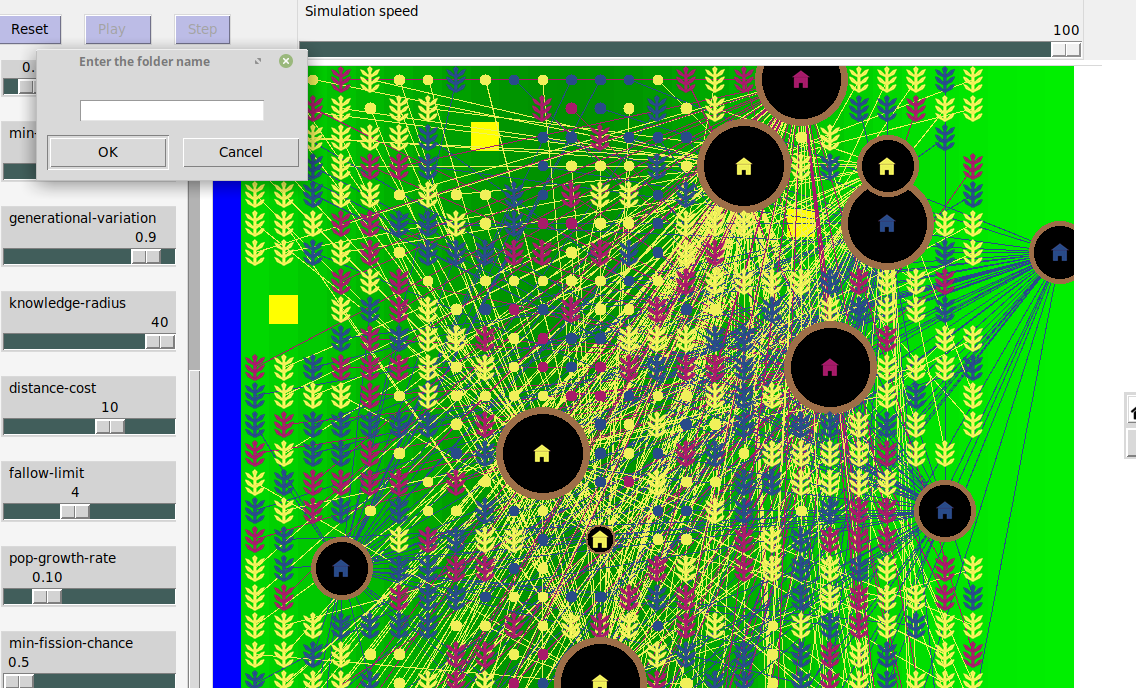
\includegraphics[width=\linewidth]{SaveAll1}
		
		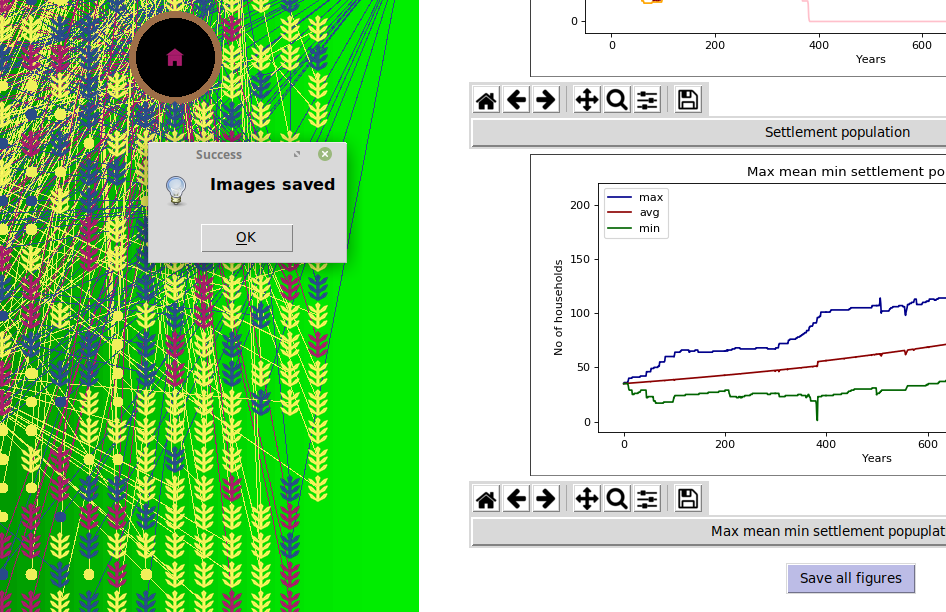
\includegraphics[width=\linewidth]{SaveAll2}
	\section{Test Cases}

	\section{Conclusions}
	
	\begin{thebibliography}{9}

	\end{thebibliography}
\end{document}